\documentclass[compress]{beamer}
\mode<presentation>

\usetheme{Warsaw}
\definecolor{innotek}{RGB}{2,52,173}
\setbeamercolor*{palette primary}{use=structure,fg=white,bg=innotek}
%\usecolortheme[RGB={2,52,173}]{structure}
\defbeamertemplate*{footline}{shadow theme}
{%
  \leavevmode%
  \hbox{\begin{beamercolorbox}[wd=.5\paperwidth,ht=2.5ex,dp=1.125ex,leftskip=.3cm plus1fil,rightskip=.3cm]{author in head/foot}%
    \usebeamerfont{author in head/foot}\hfill\insertshortauthor%
  \end{beamercolorbox}%
  \begin{beamercolorbox}[wd=.5\paperwidth,ht=2.5ex,dp=1.125ex,leftskip=.3cm,rightskip=.3cm plus1fil]{title in head/foot}%
      \usebeamerfont{title in head/foot}\insertshorttitle\hfill\insertframenumber\,/\,\inserttotalframenumber%
  \end{beamercolorbox}}%
  \vskip0pt%
}
\setbeamertemplate{navigation symbols}{}%remove navigation symbols

\usepackage{subfigure}
\usepackage{multicol}
%\usepackage{amsmath}
\usepackage{epsfig}
\usepackage{graphicx}
\usepackage[all,knot]{xy}
\xyoption{arc}
\usepackage{url}
\usepackage{multimedia}
\usepackage{hyperref}
\usepackage{setspace}

% define your own colours:
\definecolor{innotek}{RGB}{1,54,160}
\definecolor{Red}{rgb}{1,0,0}
\definecolor{Blue}{rgb}{0,0,1}
\definecolor{Green}{rgb}{0,1,0}
\definecolor{magenta}{rgb}{1,0,.6}
\definecolor{lightblue}{rgb}{0,.5,1}
\definecolor{lightpurple}{rgb}{.6,.4,1}
\definecolor{gold}{rgb}{.6,.5,0}
\definecolor{orange}{rgb}{1,0.4,0}
\definecolor{hotpink}{rgb}{1,0,0.5}
\definecolor{newcolor2}{rgb}{.5,.3,.5}
\definecolor{newcolor}{rgb}{0,.3,1}
\definecolor{newcolor3}{rgb}{1,0,.35}
\definecolor{darkgreen1}{rgb}{0, .35, 0}
\definecolor{darkgreen}{rgb}{0, .6, 0}
\definecolor{darkred}{rgb}{.75,0,0}

\xdefinecolor{olive}{cmyk}{0.64,0,0.95,0.4}
\xdefinecolor{purpleish}{cmyk}{0.75,0.75,0,0}

\useoutertheme[subsection=false]{smoothbars}

\title{POW-R}
\subtitle{Power Outlet Wireless Reporter}
\author[]{Charles Hathaway\\Grace De Geus\\Niloc Quimby\\Nate Pickett}
%\institute[Innotek]{
\includegraphics[width=20mm]{Pictures/Innotek.png}}
\date{December $7^{th}$, 2012}

\begin{document}

\frame{
    \titlepage
}

\section[Outline]{}


\section{Overview}



\section{Requirements}

\section{The People}
\subsection{What we're working on - Group}

\frame{
 \frametitle{What we're working on - Group}
 \begin{itemize}
  \item Project Concept
  \item Requirements
  \item Architectural Design
  \item Low Level Design
  \item Prototyping
  \item Development
 \end{itemize}
}
\subsection{What I'm working on - Charles}

\frame{
 \begin{itemize}
  \item Overall software architecture
  \item The server software/hardware
  \item The front-end
  \begin{enumerate}[A.]
   \item All the templates
  \end{enumerate}
  \item The back-end
  \begin{enumerate}[A.]
   \item The REST API
   \item Verifying the database (all modules)
  \end{enumerate}
 \end{itemize}
}
\subsection{What I'm working on - Grace}

\frame{
 \frametitle{What I'm working on - Grace}
 \begin{itemize}
  \item Display - Front-end
  \item Graphs  
 \end{itemize}
}
\subsection{What I'm working  on - Nate}

\frame{
 \frametitle{What I'm working on - Nate}
 \begin{itemize}
  \item Prototyping Hardware
  \item Satellite
 \end{itemize}
}

\subsection{What I'm working on - Niloc}

\frame{
 \begin{itemize}
  \item Prototyping hardware
  \item ZigBee specification  
 \end{itemize}
}



\section{Architecture}

%Nilocwords: 
% - Introduce ZigBee by first talking about its role in our project
% - Explain XBee / ZigBee relationship and differences.
\section{ZigBee}
\frame{\frametitle{ZigBee Overview}
	\begin{itemize}
		\item All inter-Satellite ("Mesh") communication
		\item Different than XBee:
			\begin{itemize}
				\item XBee is a small digital radio (Hardware)
				\item ZigBee is the specification it talks over ('Protocol')
			\end{itemize}				
	\end{itemize}
	

% - Compare specification to Bluetooth (relatable)
% - Low power, low data rate communication over digi radios
% - Explain PAN standard and why it's important
% - Explaining 'slightly' open source:
%		Open source as far as documentation and development,
%		however to be branded "ZigBee Compliant", must be member
%		of ZigBee Alliance. Has membership fee. Thus, conflicts
%		with GNU General Pub License
\subsection{What is ZigBee?}
\frame{\frametitle{What is ZigBee?}
	\begin{itemize}
		\item Specification, much like Bluetooth
		\item Low power communication over digital radios
		\item Based on 802.15.4 (PAN standard)
		\item 'Slightly' open-source
	\end{itemize}
	

% - ZigBee forms Mesh network on it's own
% 		save for some configurations in hardware
% - Explain how each feature is important to the project:
% 		Mesh is localized and encrypted (secure),
%		meaning Satellites can be safely added
%		in the target residence, quick and easy
% - Explain how ZigBee compliant devices 'bark' to each other
% 		and how adding nodes to the network expands the network's
%		effective range
\subsection{Why ZigBee?}
\frame{\frametitle{Why ZigBee?}
	\begin{itemize}
		\item Ad-hoc 'Mesh' networking
		\item Capable of adding nodes on-the-fly
		\item Localized and yet expandable network
		\item Has it's own encryption
	\end{itemize}


% - Any ZigBee Mesh has only one Coordinator,
%		which administrates and maintains Mesh.
% - Routers can send/rcv data for themselves,
%		and also route data to/from other ZigBee devices
% - End devices are super low-power, but require a
%		specific Router to be their 'parent.'
%		We aren't using these at all.
% - Explain massive amounts of radios per network
\subsection{How ZigBee Works}
\frame{\frametitle{How ZigBee Works}
	\begin{itemize}
		\item Three 'roles' in ZigBee networks:
		\begin{itemize}
			\item Coordinator
			\item Routers
			\item End-devices
		\end{itemize}
		\item Addressing scheme supports 
		\item Supports many network topologies
	\end{itemize}


% - Network types supported:
		Pair, Star, not very interesting.
%		Mesh is what we're using.
\subsection{Network Topology Examples}
\frame{\frametitle{Network Topology Examples}
\begin{figure}
\centering
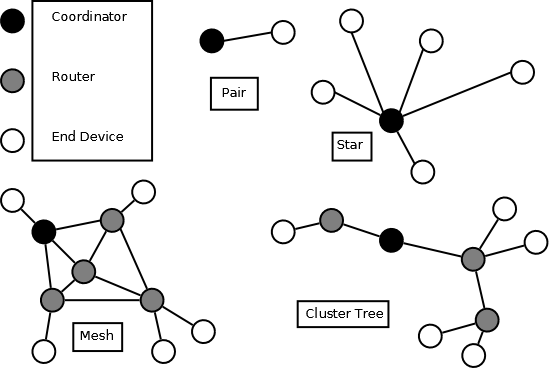
\includegraphics[scale=.8]{Diagrams/ZigBeeNetworkTypes.png}
\end{figure}
\section{Satellite}
\frame{
\frametitle{What are the Satellites?}
\begin{itemize}
\item Satellites are the devices in the outlets.
\begin{itemize}
\item Do all of the data measuring.
\end {itemize}
\end{itemize}
}


\subsection{Overview}
\frame {
 \frametitle{Satellite Overview}
\begin{center}
 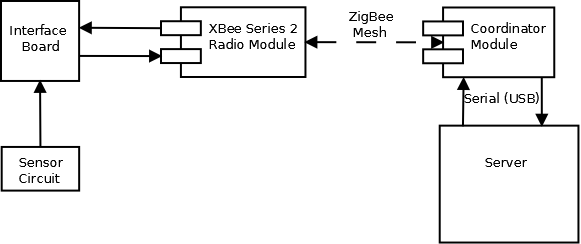
\includegraphics[width=0.8\textwidth]{Diagrams/DetailOverview.png}
\end{center}
}

\frame{
 \frametitle{Measurement Hardware}
 \begin{itemize}
 \item Current Transformer
 \end{itemize}
 \begin{center}
  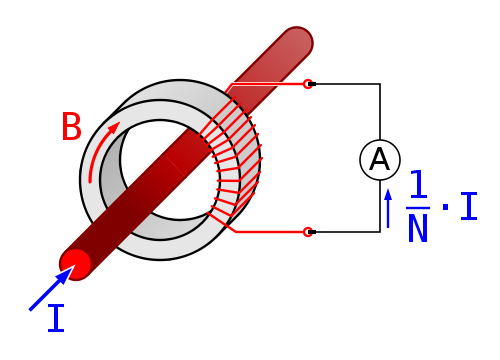
\includegraphics[width=0.8\textwidth]{Diagrams/CurrentTransformer.png}
  \end{center}
}

\section{Software}

\subsection{Overview}

\frame {
 \frametitle{Software Overview}
 \begin{itemize}
  \item Python on the backend
  \begin{enumerate}[A.]
   \item Django for the REST, HTTP stuff
   \item Custom python to interact with Arduino interface
  \end{enumerate}
  \item Heavy Javascript on the frontend
  \begin{enumerate}[A.]
   \item jqplot for creating graphs (jQuery included)
   \item RequireJS for module dependency and loading
   \item BackboneJS for MVC architecture
  \end{enumerate}
 \end{itemize}
}

\frame{
 \frametitle{Backend Overview}
 \begin{itemize}
  \item Django will be used to handle database
  \item Tastypie will be used to prototype the REST API
  \item Django admin will be used to prototype the admin interface
  \item Each functional area of the project will be a Django module
  \begin{enumerate}[A.]
   \item Power Bill Guestimator
   \item Satellite
   \item REST API
  \end{enumerate}
 \end{itemize}
}

\subsection{Interesting problems}

\frame{
 \frametitle{Power Bill Guestimator}
 \begin{itemize}
  \item Power companies have different ways of charging
  \begin{enumerate}[A.]
   \item Power consumptions tiers
   \item Prime-time vs Off-time
  \end{enumerate}
  \item Cost of power can fluctuate (over long periods of time)
  \item Need to keep a history
  \item Database-consolidation can't mix power "tiers"
 \end{itemize}
}
 
\frame{
 \frametitle{Power Bill Guestimator Solutions}
 \begin{itemize}
  \item Support all methods of charging power
  \item Store key in data table indicating what power "tier" applies
  \item Calculate current power tier at runtime
  \begin{enumerate}[A.]
   \item Scheduling problem
   \item Calculate during save for efficiency
  \end{enumerate}
 \end{itemize}
}

\frame{
 \frametitle{Limited Resources}
 \begin{itemize}
  \item Server must be low powered
  \begin{enumerate}[A.]
   \item Limited processing power
   \item Limit memory capacity
  \end{enumerate}
  \item Server must store data for years
  \item Server must be able to serve many clients
  \item Server must be online 24/7 with some reliability
  \item Server must be able to process data from all Satellites
 \end{itemize}
}

\frame{
 \frametitle{Limited Resources Solution}
 \begin{itemize}
  \item Bare-bones operating system
  \item Compacting database
  \item Offload templating to clients via Javascript
  \begin{enumerate}[A.]
   \item REST API
   \item JSON
  \end{enumerate}
  \item Use well-known and tested components
  \item Use a database which supports simultaneous read/writes
 \end{itemize}
}

\frame{
 \frametitle{Limited Time}
 \begin{itemize}
  \item We have 2 software engineers, not full time
  \item We have 3 computer engineers, not full time
  \begin{enumerate}[A.]
   \item Most focus on the hardware
  \end{enumerate}
  \item Lots of implied requirements
  \begin{enumerate}[A.]
   \item Access control
   \item Extensible API
   \item History tables
  \end{enumerate}
 \end{itemize}
}

\frame{
 \frametitle{Limited Time - Solutions}
 \begin{itemize}
  \item Modular - Prototype components with the expectation of complete replacements
  \item Open Source - Utilize free libraries
  \item One stone for many birds
  \begin{enumerate}[A.]
   \item Use this project for other classes
   \item Use architecture and design that we're familiar with
   \item Reusable components
  \end{enumerate}
 \end{itemize}
}

\section{Conclusions}

\frame{
    \begin{center}
        {\huge Questions?}
    \end{center}
}


\end{document}

